\documentclass[a4paper,12pt]{article} 

% packages and main settings
\usepackage[left=3cm, right=2cm, top=2cm, bottom=2cm]{geometry}
\usepackage[english]{babel}    
\usepackage[utf8]{inputenc}  
\usepackage[T1]{fontenc}        
\usepackage{lmodern}            
\usepackage{microtype}          
\usepackage{amsmath}
\usepackage{amsfonts, amsthm, amssymb, graphicx, booktabs}
\usepackage{bm} %bold epsilon
\usepackage{newclude}   
\usepackage{placeins}  %surpresses floating tables
\usepackage[labelfont=bf]{caption} %Figure etc steht dann in small caps 
\usepackage[labelsep=period]{caption} % dot after figure, table caption.
\usepackage[flushleft]{threeparttable} % for notes below table
\usepackage{multirow} % for table cell merge along rows
\usepackage{graphicx} % to adjust tablesize to textwidth
\usepackage{caption}  % for centered captions
\usepackage{float} % to set of autopositioning of tables
\usepackage[bottom,hang,flushmargin]{footmisc} % forces footnotes to the bottom
\usepackage{setspace}           % Fuer 1.5 fachen Zeilenabstand  
\onehalfspacing % 1.5 cm Zeilenabstand
%Bibtex
\usepackage[round,sort&compress]{natbib}

\bibliographystyle{chicago} % chicago bib style like in AER
\usepackage[hidelinks]{hyperref} % fuer links und verweise. Cleverref ist eigentlich besser. 


% Create header. The header must be surpressed for 
% every first page per section and a solution
% for the Appendix is used in the respective subfile.
\usepackage{fancyhdr}
\pagestyle{fancy}
\fancyhf{}
\chead{\nouppercase{\textit{\leftmark}}}
\cfoot{\thepage}
\renewcommand{\headrulewidth}{0pt} % no vertical line

%\usepackage{lipsum}  % check if formats work

\usepackage{afterpage} %clearpage w/o pagebreak for "header bug"

% Expectation symbol
\DeclareMathOperator*{\E}{\mathbb{E}}

% thin space, limits underneath in displays
% for strike through
\DeclareMathOperator*{\argmax}{argmax}
\newcommand*{\defeq}{\stackrel{\text{def}}{=}}
\usepackage[normalem]{ulem}
% try to use strikeout in section headers and others
\DeclareRobustCommand{\hsout}[1]{\texorpdfstring{\sout{#1}}{#1}}

% for gray table row color
\usepackage[table]{xcolor}

% decimal dot alignment in table columns
\usepackage{siunitx}

% for footnotes in table
\usepackage[flushleft]{threeparttable}

% for underbar
\newcommand{\ubar}[1]{\text{\b{$#1$}}}

\usepackage{tikz}

% Setup for urls
\usepackage{url}

\defcitealias{Respy-Stenzel.2019}{\textit{respy}}
\defcitealias{Gabler.2019}{\textit{estimagic}}
\defcitealias{Stenzel.2020}{\textit{Master's Thesis Replication Repository}}
\defcitealias{NLSY79}{NLSY79}


\usepackage{tikz}


\usepackage{enumitem}



\begin{document}

\newpage % delete after section is complete

\section{Qualitative GSA measures for functions with correlated input parameters}
\thispagestyle{plain} % suppress header on first page

\subsection{Qualitative General Sensitivity Analysis}
\noindent
Qualitative Global Sensitivity Analysis (Qualitative GSA) deals with computing measures that can rank random input parameters in terms of their impact on the function output and the variability thereof. If the measures for some input parameters are negligibly small, these parameters can be fixed so that the number of random input parameters decreases for a subsequent quantitative GSA. This pre-selection step is called Factor Fixing. The quantitative GSA then aims to determine the precise effect size of each random input parameter on the function output. The most common measures in quantitative GSA are the so-called Sobol' sensitivtiy indices. Equation 1 shows the first order index. It is the share of the variance in the function output induced by exclusively one single input parameter $X_i$ of the variance induced by all random input parameters $X_1, X_2, ..., X_k$.


\begin{align}
S_i = \frac{\text{Var}_i[Y|X_i ]}{\text{Var}[Y]}
\end{align}

\noindent
Let $\sim i$ denote the set of indices except $i$. Equation 2 shows the total order index. This measure is equal to the first order index except of that its numerator includes the variance in the function output that is induced by changes in the other input parameters $X_{\sim i}$, caused by interactions with the variation in $X_i$.

\begin{align}
S_{i}^T = \frac{\E_{\sim i}[\text{Var}_{i}[Y|\bold{X_{\sim i}]]}}{\text{Var}[Y]}
\end{align}

\noindent
Computing these measures requires many function evaluations, even if an estimator is used as a shortcut. The more time-intense one function evaluation is, the more utility provides the aforementioned Factor Fixing based on qualitative measures. The most commonly used measures in qualitative GSA is the mean Elementary Effect (EE), $\mu$, the mean absolute Elementary Effects, $\mu^*$, and the standard deviation of the Elementary Effects, $\sigma$. The Elementary Effect of $X_i$ is given by one individual function derivative with respect to $X_i$. The "change in", or the "step of" the input parameter, denoted by $\Delta$, has not to be infinitesimally small. The only restriction is that $X_i + \Delta$ is in the domain of $X_i$. The Elementary Effect, or derivative, is denoted by
\begin{align}
d_i^{(j)} =  \frac{Y(\bold{X_{\sim i}^{(j)}}, X_i^{(j)} + \Delta^{(i,j)})}{\Delta^{(i,j)}},
\end{align}
where $j$ is an index for the number of $r$ observations of $X_i$.
Then, the mean Elementary Effect is given by

\begin{align}
\mu_i = \frac{1}{r} \sum_{j=1}^{r} d_i^{(j)}.
\end{align}
\noindent
The mean absolute Elementary Effect, $\mu_i^*$ is used to prevent observations of opposite sign to cancel each other out:

\begin{align}
\mu_i^* = \frac{1}{r} \sum_{j=1}^{r} \big| d_i^{(j)} \big|.
\end{align}
\noindent
Step $\Delta^{(i,j)}$ may or may not vary depending on the sample design that is used to draw the input parameters. These measures (together) are used to proxy the total Sobol' indices that contains the parameter-specific interactions with all other parameter, as shown in Equation (2). The total Sobol' index is the relevant one because the interactions are potentially be important. If the qualitative measures are close to 0 for one particular parameter, its variation can be rendered as irrelevant for the variation in the function output (given there are parameters with measures substantially different from 0).

\subsection{Sampling Schemes}

According to several experiments by \cite{campolongo2011screening} using common test functions, the best design is the radial design (\cite{saltelli2002making}) and the most commonly used is the trajectory design (\cite{Morris.1991}).
Both designs are comprised by a $(k + 1) \times k$-dimensional matrix. The elements are generated in $[0,1]$. Afterwards, they can potentially be transformed to the distributions of choice. The columns represent the different input parameters and each row is a complete input parameter vector. To compute the aggregate qualitative measures, a set of multiple matrices, or subsets, of input parameters has to be generated.\\

\noindent
A matrix in radial design is generated the following way: Draw a vector of length $2k$ from a quasi-random sequence. The first row, or parameter vector, is the first half of the sequence. Then, copy the first row to the remaining $k$ rows. For each row $k'$ of the remaining 2, ..., $k+1$ rows, replace the $k'$-th element by the $k'$-th element of the second half of the vector. This generates a matrix of the following form:
\begin{align}
\underset{(k+1)\times k}{\bold{R}} =
\begin{pmatrix}
a_1 & a_2 & ... & a_k \\
\bold{b_1} & a_2 & ... & a_k \\
a_1 & \bold{b_2} & ... & a_k \\
\vdots & \vdots & 	\ddots & \vdots\\
a_1 & a_2 & ... & \bold{b_k}
\end{pmatrix}
\end{align}
\noindent
Note here, that each column consists only of the first row element, except of for one row.
From this matrix, one EE can be obtained for each parameter $X_i$. This is achieved by using the $(i+1)$-th row as function argument for the minuend and the first row as subtrahend in the formula for the EE. Then, $\Delta^{(i,j)} = b_i^{(j)} - a_i^{(j)}$. Tailored to the radial scheme, the derivative can be re-formulated as in Equation (3), where $i$ represents the input parameter $X_i$. We abstract from multiple sample sets and do not use index $j$ compared to Equation (3). The asterisk is an index for a complete vector.
\begin{align}
d_i =  \frac{Y(\bold{a_{\sim i}}, b_i) - Y(\bold{a})}{b_i - a_i} = \frac{Y(\bold{R_{i+1,*}}) -  Y(\bold{R_{1,*}})}{b_i - a_i}.
\end{align}
If the number of radial subsamples is high, the draws from the quasi-random sequence lead to a good and fast coverage of the input space (compared to a random sequence). The quasi-random sequence considered here is the Sobol' sequence. This sequence is comparably succesful in covering the unit hypercube, but also conceptually more involved. Therefore, its presentation is beyond the scope of this work. Since this sequence is quasi-random, the sequence has to be drawn at once for all sets of radial matrices.\\

\noindent
Next, I present the trajectory design. As we will see, it leads to a relatively representative coverage for a very small number of subsamples but also to frequent repetitions of similar draws.
In this outline, I skip the equations that generate a trajectory and present the method verbally.
There are different forms of trajectories. Here, I focus on the version presented in \cite{Morris.1991} that yields to equiprobable elements. The first step is to decide the number $p$ of equidistant grid points in interval $[0,1]$. Then, the first row of the trajectory is composed of the lower half value of these grid points. Now, fix $\Delta = p/[2(p-1)]$. This function implies, that adding $\Delta$ to the lowest point in the lowest half results in the lowest point of the upper half of the grid points, and so on. The rest of the rows is constructed by, first, copying the row one above and, second, by adding $\Delta$ to the $i$-th element of the $i+1$-th row. The implied matrix scheme is depicted below.
\begin{align}
\underset{(k+1)\times k}{\bold{T}} =
\begin{pmatrix}
a_1 & a_2 & ... & a_k \\
\bold{b_1} & a_2 & ... & a_k \\
\bold{b_1} & \bold{b_2} & ... & a_k \\
\vdots & \vdots & 	\ddots & \vdots\\
\bold{b_1} & \bold{b_2} & ... & \bold{b_k}
\end{pmatrix}
\end{align}
\\

\noindent
In contrary to the radial scheme, each $b_i$ is copied to the subsequent row. Therefore, the EEs have to be determined by comparing each row with the row above instead of with the first row.
Importantly, two random transformations are common. These are randomly switching rows and randomly interchanging the $i$-th column with the $(k-i)$-th column and then reversing the column. The first transformation is skipped as it does not add additional coverage and because we need the stairs-shaped design to facilitate later transformations which account for correlations between input parameters. The second transformation is adapted because it is important to also have negative steps and because it does sustain the stairs shape. Yet, this implies that $\Delta^{(i)}$ is also parameter- and trajectory-specific. Let $f$ and $h$ be additional indices representing the input parameters. The derivative formula is adapted to the trajectory design as follows:\footnote{In contrary to most authors, I also denote the step as a subtraction instead of $\Delta$ when referring to the trajectory design. This provides additional clarity.}

\begin{align}
d_i =  \frac{Y(\bold{b_{f \leq i}}, \bold{a_{h>i}}) - Y(\bold{b_{f<i}}, \bold{a_{h \geq i}})}{b_i - a_i} = \frac{Y(\bold{T_{i+1,*})} -  Y(\bold{T_{i,*}})}{b_i - a_i}.
\end{align}
The trajectory design involves first, a fixed grid, and second and more importantly, a fixed step $\Delta$. s.t. $\{\Delta\} = \{\pm \Delta\}$. This implies less step variety and less space coverage vis-á-vis the radial design for more than a small number of draws.\\

\noindent
So far, we have only considered draws in [0,1]. For uncorrelated input parameters from arbitrary distributions with well-defined cumulative distribution function, $\Phi$, one would simply evaluate each element (of course, potentially including the addition of the step) by the inverse cumulative distribution function, $\Phi^{-1}$, of the respective parameter. A bit of intuition is, that $\Phi$ maps the sample space to [0,1]. Hence $\Phi^{-1}$ can be used to transform random draws in [0,1] to the sample space of the arbitrary distribution. This is a basic example of so-called inverse transform sampling which we will recall in the next section.



\subsection{The approach for correlated input parameters in \cite{ge2017extending}}

This section describes the incomplete approach by \cite{ge2017extending} to extend the EE-based measures to input parameters that are correlated. Their main achievement is to outline a transformation of samples in radial and trajectory design that incorporates the correlation between the input parameters. This implies, that the trajectory and radial samples cannot be written as in Equation (6) and Equation (8). The reason is that the correlations of parameter $X_i$, to which step $\Delta^i$ is added, implies that all other parameters in the same row with non-zero correlation in $\bold{X_{\sim i}}$ are changed as well. Therefore, the rows cannot be denoted and compared as easily by $a$'s and $b$'s as in Equation (6) and (8). Transforming these matrices allows to re-define the EE-based measures accordingly, such that they sustain the main properties of the ordinary measures for uncorrelated parameters. The property is being a function of the mean derivative. Yet, \cite{ge2017extending} fail to fully develop these measures. I will explain how their measures lead to arbitrary results for correlated input parameters. This section covers their approach in a simplified form, focussing on normally distributed input parameters, and presents their measures.\\

\noindent
The next paragraph deals with developing a recipe for transforming draws $\bold{u} = \{u_1, u_2, ..., u_k\}$ from $[0,1]$ for an input parameter vector to draws $\bold{x} = \{x_1, x_2, ..., x_k\}$ from an arbitrary joint normal distribution. We will do this in three steps. 

For this purpose, let $\bold{\Sigma}$ be a non-singular variance-covariance matrix and let $\pmb{\mu}$ be the mean vector. The $k$-variate normal distribution is denoted by $\mathcal{N}_k(\pmb{\mu}, \bold{\Sigma})$. \\

\noindent
Creating potentially correlated draws $\bold{x}$ from $\mathcal{N}_k(\pmb{\mu}, \bold{\Sigma})$ is simple. Following \cite{gentle2006random}, page 197, this can be achieved the following way: Draw a $k$-dimensional row vector of i.i.d standard normal deviates from the \textit{univariate} $N_1(0,1)$ distribution, such that  $\bold{z} = \{z_1, z_2, ..., z_k\}$, and compute the Cholesky decomposition of $\Sigma$, such that $\bold{\Sigma} = \bold{T^T T}$. The lower triangular matrix is denoted by $\bold{T^T}$. Then apply the operation in Equation (10) to obtain the correlated deviates from $\mathcal{N}_k(\pmb{\mu}, \bold{\Sigma})$.
\begin{align}
\bold{x} = \pmb{\mu} + \bold{T^T z^T} 
\end{align}
Intuition for the mechanics  that underlie is provided in Appendix A (not contained in this draft). \\

\noindent
The next step is to understand that we can split the operation in Equation (10) into two subsequent operations. For this, let $\pmb{\sigma}$ be the vector of standard deviations and let $\bold{R_k}$ be the correlation matrix of $\bold{x}$.

The first operation is to transform the standard deviates $\bold{z}$ to correlated standard deviates $\bold{z_c}$ by using $\bold{z_c}=\bold{Q^T z^T}$. In this equation, $\bold{Q^T}$ is the lower matrix from the Cholesky decomposition $\bold{R_k}=\bold{Q^T Q}$. This is equivalent to the above approach in \cite{gentle2006random} for the specific case of the multivariate standard normal distribution $\mathcal{N}_k(0, R_k)$. This is true because for multivariate standard normal deviates, the correlation matrix is equal to the covariance matrix.

The second operation is to scale the correlated standard normal deviates: $\bold{z}=\bold{z_c(i)}\pmb{\sigma}\bold{(i)} + \pmb{\mu}$., where the $i$s indicate an element-wise multiplication.\\

\noindent
The last step to construct the final approach is to recall the inverse transform sampling method. Therewith, we can transform the input parameter draws $\bold{u}$ to uncorrelated standard normal draws $\bold{z}$. Then we will continue with the two operation in the above paragraph. The transformation from $\bold{u}$ to $\bold{z}$ is denoted by $ F^{-1}(\Phi)$ and summarized by the following three points:


\[
\left.\parbox{0.5\textwidth}{%
\begin{enumerate}[label=\bfseries Step \arabic*:,leftmargin=*,labelindent=5em]
	\item $\bold{z} = \pmb{\Phi^{-1}({u})}$
    \item $\bold{z_c} = \bold{Q^T z^T}$
    \item $\bold{x} = \pmb{\mu} + \bold{z_c(i)}\pmb{\sigma(i)}$
\end{enumerate}
}\right\}F^{-1}(\Phi) \defeq \mathcal{T}_2
\]

Step 3 is specific to the normal sample space in which we are interested in. A mapping to other sample spaces can, for instance. be achieved by, first, applying $\Phi$ and, second, the inverse cumulative distribution function of the desired distribution.

\noindent
The procedure described in the three steps above is equivalent to an inverse Rosenblatt transformation, a linear inverse Nataf transformation\footnote{For the first two transformations, see \cite{lemaire2013structural}, page 78 - 113} and connects to Gaussian copulas. These concepts can be used to transform deviates in [0,1] to the sample space of arbitrary distributions by using the properties sketched above under varying assumptions. Notes on this relation are provided in Appendix B (not contained in this draft).\\

\noindent
The one most important point to understand is that the transformation comprised by the three steps listed above is not unique for correlated input parameters. Rather, the transformation changes with the order of parameters in vector $\bold{u}$ (see also the formal definition of the Rosenblatt transformation). This can be seen from the lower triangular matrix $\bold{Q^T}$. To prepare the next equation, let $\bold{R_k} = (\rho_{ij})_{ij=1}^k$ and sub-matrix $\bold{R_h} = (\rho_{ij})_{ij=1}^h$, $h \leq k$. Also let $\pmb{\rho_i^{*,j}} = (\rho_{1,j}, \rho_{2,j}, ..., \rho_{i-1,j})$ for $j \geq i$ with the following abbreviation $\pmb{\rho_i}\defeq\pmb{\rho_i^{*,i}}$. Following \cite{madar2015direct}, the lower matrix can be written as

\begin{align}
\bold{Q^T} =
\begin{pmatrix}
\\ 1 & 0 & 0 & ... & 0
\\\rho_{1,2} & \sqrt{1-\rho_{1,2}^2} & 0 & ... & 0
\\ \rho_{1,3} & \frac{\rho_{2,3}-\rho_{1,2}\rho_{1,3}}{\sqrt{1-\rho_{1,2}^2}} & \sqrt{1-\pmb{\rho_{3}}\bold{R^{-1}_2}\pmb{\rho_{3}^T}} & ... & 0
\\\vdots & \vdots & \vdots & 	\ddots & \vdots
\\ \rho_{1,k} &\frac{\rho_{2,k}-\rho_{1,2}\rho_{1,k}}{\sqrt{1-\rho_{1,2}^2}} & \frac{\pmb{\rho_{3,k}}-\pmb{\rho_{3}^{*,k}}\bold{R^{-1}_2}\pmb{\rho_{3}^T}}{\sqrt{1-\pmb{\rho_{3}}\bold{R^{-1}_2}\pmb{\rho_{3}^T}}}  &
... & \sqrt{1-\pmb{\rho_{k}}\bold{R^{-1}_2}\pmb{\rho_{k}^T}}
\end{pmatrix}.
\end{align}
Equation (11), together with Step 2, implies that the order of the uncorrelated standard normal deviates $\pmb{z}$ constitute a hierarchy amongst the correlated deviates $\bold{z_c}$, in the following manner: The first parameter is not subject to any correlations, the second parameter is subject to the correlation with the first parameter, the third parameter is subject to the correlations with the parameters before, etc. Therefore, if parameters are correlated, typically $\bold{Q^T z^T} \neq \bold{Q^T (z')^T}$ and $F^{-1}(\Phi)(\bold{u}) \neq F^{-1}(\Phi)(\bold{u'})$, where $\bold{z'}$ and $\bold{u'}$ denote $\bold{z}$ and $\bold{u}$ in different orders. One could say that the correlations are transferred like the fall of dominoes.

Coming back to the EE-based measures for correlated inputs, \cite{ge2017extending} attempt to construct two variations of derivatives / EEs, $d$, in Equation (3). They call one derivative the independent Elementary Effects, $d_i^{ind}$, and the other the full Elementary Effects, $d_i^{full}$. For each of these two EEs, they derive the aggreate measures $\mu$, $\mu^*$ and $\sigma$. The difference between the two EEs is, that $d^{ind}$ excludes and $d^{full}$ includes the effect of the correlations from adding the step $\Delta^i$ to $X_i$ on the other parameters $\bold{X_{\sim i}}$. Knowing $d_i^{ind}$ is important because the correlations can decrease $d_i^{full}$ (close to 0). However, if the independent-EE-based measures are not close to zero, $X_i$ is still important. Additionally, fixing this parameter might possibly change the $d_i^{full}$s of $\bold{X_{\sim i}}$.\\

\noindent 
For the trajectory design, the formula for the full Elementary Effect, is given by
\begin{align}
d_i^{full,T} = \frac{f\big(\mathcal{T}(\bold{T_{i+1,*}}; i-1)\big) - f\big(\mathcal{T}(\bold{T_{i,*}}; i)\big)}{\Delta}.
\end{align}
In Equation (12), $\mathcal{T}(\cdot; i) \defeq \mathcal{T}_3\bigg(\mathcal{T}_2\big(\mathcal{T}_1(\cdot; i)\big); i\bigg)$. $\mathcal{T}_1(\cdot; i)$ orders the parameters / row elements to establish the right correlation hierarchy. $\mathcal{T}_2$, or $F^{-1}(\Phi)$, correlates the draws in $[0,1]$ and transforms them to the sample space. $\mathcal{T}_3(\cdot; i)$ reverses the element order back to the start, to be able to apply the subtraction in the numerator of the EEs row-by-row. Index $i$ in $\mathcal{T}_1(\cdot; i)$ and $\mathcal{T}_3(\cdot; i)$ stands for the number of first row elements that is cut and moved to the back of the row in the same order and the reverse transformation. Applying $\mathcal{T}(\bold{T_{i+1,*}}; i-1)$ and $\mathcal{T}(\bold{T_{i+1,*}}; i)$ to all rows $i$ of trjactory $\bold{T}$ as in Equation (12) yields the following two transformed trajectories:

\begin{align}
\mathcal{T}_1(\bold{T_{i+1,*}}; i-1)
=
\begin{pmatrix}
a_k & a_1 & ... & ... &  a_{k-1} \\
\bold{b_1} & a_2 & ... & ... &  a_k \\
\bold{b_2} & a_3 & ... & ... &  \bold{b_1} \\
\vdots & \vdots & \vdots & 	\ddots &  \vdots\\
\bold{b_k} & \bold{b_{1}} & ... & ... &  \bold{b_{k-1}}
\end{pmatrix}
\end{align}
\begin{align}
\mathcal{T}_1(\bold{T_{i,*}}; i-1)=
\begin{pmatrix}
a_1 & a_2 & ... & ... &  a_k \\
a_2 & ... & ... &  a_k & \bold{b_1} \\
a_3 & ... & ... &  \bold{b_1} & \bold{b_2} & \\
\vdots & \vdots & \vdots & 	\ddots &  \vdots\\
\bold{b_1} & \bold{b_{2}} & ... & ... &  \bold{b_{k}}
\end{pmatrix}
\end{align}
Two points can be seen from Equation (13) and (14). First, $\mathcal{T}_1(\bold{T_{i+1,*}}; i-1)$ and $\mathcal{T}_1(\bold{T_{i,*}}; i)$, i.e. the $(i+1)$-th row in Eq. (13) and the $(i)$-th row in Eq. (14) only differ in the $(i)$-th element. The difference is $b_i - a_i$. Thus, these two rows can be used to compute the Elementary Effects as for the uncorrelated case in Equation (9). However, in this order, the parameters are in the wrong positions to be directly handed over to the function, as the $i$-th parameter is always in front. The second point is that in $\mathcal{T}_1(\bold{T_{i+1,*}}; i-1)$, $b_i$ is in front of the $i$-th row. This order prepares the establishing of the right correlation hierarchy by $\mathcal{T}_2$, such that the $\Delta$ in $a_i + \Delta$ is included to transform all other elements that represent parameters $X_{\sim i}$. Importantly, to perform $\mathcal{T}_2$, the mean vector $\bold{x}$ and the covariance matrix $\pmb{\Sigma}$ and its transformed representatives have always to be re-ordered according to each row. 
Then, $\mathcal{T}_3$ restores the original row order and $d_i^{full}$ can comfortably be computed by comparing function evaluations of row $i+1$ in $\mathcal{T}(\bold{T_{i+1,*}}; i-1)$ with function evaluations of row $i$ in $\mathcal{T}(\bold{T_{i,*}}; i-1)$. Now, the two transformed trajectories only differ in the $i$-th element in each row $i$. \\

\noindent
The formula for the independent Elementary Effect for the trajectory design is given by
\begin{align}
d_i^{ind, T} = \frac{f\big(\mathcal{T}(\bold{T_{i+1,*}}; i)\big) - f\big(\mathcal{T}(\bold{T_{i,*}}; i)\big)}{\Delta}.
\end{align}

Note that $\mathcal{T}(\bold{T_{i+1,*}}; i) = \mathcal{T}(\bold{T_{i,*}}; i-1)$ which is the funcion argument in the subtrahent in the definition of $d^{full}$ in Equation (12). Therefore this transformation can be skipped for the trajectory design and the transformed trajectory in Equation (14) can be recycled. Here, the $X_i$ that takes the step in the denominator of the Elementary Effect is moved to the back such that the step does not affect the other input parameters $\bold{X_{\sim i}}$ through the correlations. The left trajectory is constructed such that for each row $i$, $a_i$ does take the step that $b_i$ took in the aforementioned minuend trajectory. The argument of the subtrahend in the denominator in $d_i^{ind}$ is given by the rows in

\begin{align}
\mathcal{T}_1(\bold{T_{i,*}}; i-1)=
\begin{pmatrix}
a_2 & a_3 & ... & ... &  a_1 \\
a_3 & ... & a_k &  \bold{b_1} & a_2 \\
a_4 & ... & \bold{b_1} &  \bold{b_2} & a_3 & \\
\vdots & \vdots & \vdots & 	\ddots &  \vdots\\
\bold{b_2} & \bold{b_{3}} & ... & ... &  \bold{b_{1}}
\end{pmatrix}
\end{align}

\noindent
The transformation for the samples in radial design work equally except of that the minuend samples are composed of the first row copied to each row below because the steps in the radial design are always taken from the draws in the first row. It is important to also reorder the minuend trajectories to account for the correlation hierarchy and the transformation to the sample space performed by $\mathcal{T}_2$. The forumalae of the Elementary Effects for the radial design are given by Equation (17) and (18).

\begin{align}
d_i^{full, R} = \frac{f\big(\mathcal{T}(\bold{R_{i+1,*}}; i-1)\big) - f\big(\mathcal{T}(\bold{R_{1,*}}; i)\big)}{b_i - a_i}.
\end{align}

\begin{align}
d_i^{ind, R} = \frac{f\big(\mathcal{T}(\bold{R_{i+1,*}}; i)\big) - f\big(\mathcal{T}(\bold{R_{1,*}}; i)\big)}{b_i - a_i}.
\end{align}

\subsection{Implementation}

I implemented the method by \cite{ge2017extending} in Python 3. I wrote at least one test for each function. This is a coverage of 100 \%. I am able to replicate their results for the normally distributed examples, i.e. Test Case 1 and Test Case 2 up to a reasonable degree given that they do not use a large number of samples.
The replication can be found in the two notebooks at branch $\textit{replication\_gm17}$.

In the next section, I will present the shortcomings of the Elementary Effects in \cite{ge2017extending}. There, I will explain why it not possible to solve common tests function for uncorrelated, normally distributed parameters.

I will also present improved measures that I created. With these, I can solve all test functions for uncorrelated and correlated normalinput parameters and uncorrelated parameters in [0,1]. Test functions that I solved exactly are, first, the large test function with six paramters in [0,1] based on the so-called $g$-function, presented in \cite{Saltelli.2008}, page 123 - 129. The second test function is the linear function with two normally distributed input parameters and non-unit variance in \cite{Smith.2014}, page 335. This function is similar to Test Case 1 and 2 and provides intuition on what the results for well-defined Elementary Effects for correlated input parameters should be. I am able to generate these results with the implementation of my measures.

\subsection{Drawbacks in \cite{ge2017extending} and Corrected Elementary Effects.}

The drawback in the definition of the Elementary Effects is that the step is transformed in the numerator multiple times but not in the denominator. Therefore, these measures are not Elementary Effects in the sense of a derivation. The transformation in the numerator is performed by applying $F^{-1}(\Phi)$ to $u_i^j = a_i^j + \Delta^{(i,j)}$. The corrected and slightly renamed measures are the correlated and the uncorrelated Elementary Effects $d_i^{c}$ and $d_i^{u}$. They are given below for arbitrary input distributions and for samples in trajectory and radial design. Let ${Q^T}_{k,*k-1}$ be the last row except of the last element of the lower triangular Cholesky matrix of the correlation matrix in the respective order of $\mathcal{T}_1(\bold{T_{i+1,*}}; i-1)$ and $\mathcal{T}_1(\bold{T_{i+1,*}}; i-1)$. Let ${Q^T}_{k,k}$ be the last element of the same matrix. Let $F^{-1}$ be a transformation that maps standard normal deviates to an arbitrary sample space. Index $*k-1$ represent all elements except of the last one of a vector of length $k$. Index $j$ is used to indicate an element-wise multiplication. Then

\begin{align}
d_i^{c,T} = \frac{f\big(\mathcal{T}(\bold{T_{i+1,*}}; i-1)\big) - f\big(\mathcal{T}(\bold{T_{i-1,*}}; i)\big)}{F^{-1}\big(\Phi(b_i)\big) - F^{-1}\big( \Phi(a_i)\big)}
\end{align}

\begin{align}
d_i^{u, T} = \frac{f\big(\mathcal{T}(\bold{T_{i+1,*}}; i)\big) - f\big(\mathcal{T}(\bold{T_{i,*}}; i)\big)}{F^{-1}\big({Q^T}_{k,*k-1}(j)T_{i+1,*k-1}^T(j) + {Q^T}_{k,k} \Phi(b_i)\big) - F^{-1}\big({Q^T}_{k,*k-1}(j)T_{i,*k-1}^T(j)+{Q^T}_{k,k} \Phi(a_i)\big)}
\end{align}

\begin{align}
d_i^{c, R} = \frac{f\big(\mathcal{T}(\bold{R_{i+1,*}}; i-1)\big) - f\big(\mathcal{T}(\bold{R_{1,*}}; i-1)\big)}{F^{-1}\big( \Phi(b_i)\big) - F^{-1}\big( \Phi(a_i)\big)}
\end{align}

\begin{align}
d_i^{u, R} = \frac{f\big(\mathcal{T}(\bold{R_{i+1,*}}; i)\big) - f\big(\mathcal{T}(\bold{R_{1,*}}; i)\big)}{F^{-1}\big({Q^T}_{k,*k-1}(j)R_{i+1,*k-1}^T(j) + {Q^T}_{k,k} \Phi(b_i)\big) - F^{-1}\big({Q^T}_{k,*k-1}(j)R_{i,*k-1}^T(j)+{Q^T}_{k,k} \Phi(a_i)\big)}.
\end{align}

\noindent
In Equation (22), ${Q^T}_{k,*k-1}(j)R_{i,*k-1}^T(j)$ refers to the transformed trajectory of the copied first rows, $\mathcal{T}(\bold{R_{i+1,*}}; i)$, as described in the previous section.

The denominator of the correlated Elementary Effect, $d_i^{c}$, consists of $\Phi$ and $F^{-1}$. These functions account for the transformation from uniform to arbitrary sample space. In $d_i^{c}$, the denominator must not account for a correlating transformation of $a_i$ and $b_i$ because ${Q^T}_{1,*} = (1, 0, 0, ..., 0)$.  Therefore, $b_i$ and $a_i$ are multiplied by one in the correlation step of the standard normal deviates.

The last point is not true for the uncorrelated Elementary Effect $d_i^{c}$. One accounts for the correlation step by multiplying $\Phi(b_i)$ by ${Q^T}_{k,*k-1}(j)T_{i+1,*k-1}^T(j)/\Phi(b_i)+{Q^T}_{k,k}$. The respective operation is done for $\Phi(b_i)$. Not accounting for $Q_t$ like \cite{ge2017extending} leads to arbitrarily decreased independent Elementary Effects for input parameters with higher correlations. As $d_i^{full}$ and $d_i^{ind}$ are interpreted jointly, both measures are in fact useless.

For $X_1, ..., X_k \sim \mathcal{N}_k(\pmb{\mu}, \bold{\Sigma})$, the denominator of $d_i^{u, R}$ simplifies drastically to

\begin{align}
\begin{split}
 \big(\mu_i + \sigma_i\big({Q^T}_{k,*k-1}(j)T_{i+1,*k-1}^T(j) + {Q^T}_{k,k} \Phi(b_i)\big) \\-  \big(\mu_i + \sigma_i\big({Q^T}_{k,*k-1}(j)T_{i+1,*k-1}^T(j) + {Q^T}_{k,k} \Phi(a_i)\big)\\= \sigma_i{Q^T}_{k,k}\big(\Phi(b_i)-\Phi(a_i)\big).
 \end{split}
\end{align}

\subsection{Replication and Validation}

Let $f(X_1, ..., X_k)$ = $\sum_{i = 1}^{k} c_i X_i$ be an arbitrary linear function. Let $\rho_{i,j}$ be the linear correlation between $X_i$ and $X_j$. Then, for all $i \in 1, ..., k$,
\begin{align}
d_i^{u,T} = d_i^{u,R} = c_i \\
d_i^{c,T} = d_i^{c,R} = \sum_{j = 1}^{k} \rho_{i,j} c_{j}.
\end{align}
This implies that the mean and the mean absolute aggregate effects are equal to their respective (individual) uncrrelated and correated Elementary Effect and that the respective standard deviation for both Elementary Effects is 0. This corresponds to the uncorrelated example in \cite{Saltelli.2008}, page 123.

\newpage
% Please add the following required packages to your document preamble:
% \usepackage{booktabs}
\setlength{\tabcolsep}{12pt} %from 6
\begin{table}[H]
	\centering
	\caption{Replication and validation for test case 1 - trajectory design}
	\label{tab:my-table}
		\renewcommand{\arraystretch}{1.2}%
	\begin{tabular}{cS[table-format=3.2]S[table-format=3.2]S[table-format=3.2]S[table-format=3.2]}
		\toprule
		{Measure}     & {GM'17}   & {Repl. $\mu^{*}$} & {Repl. $\sigma$} & {S'20} \\ \midrule


		& 1.20  & 1.36         & 0.83         & 1.00 \\
		\qquad $\mu^{*,ind}$                               & 1.30  & 1.48         & 0.91         & 1.00 \\
		& 3.20  & 3.11         & 1.94         & 1.00 \\
						&&&& \\
		& 0.55  & 0.00         & 0.56         & 0.00 \\
		\qquad $\sigma^{ind}$                            & 0.60  & 0.00         & 0.62         & 0.00 \\
		& 1.30  & 0.00         & 1.32         & 0.00 \\
						&&&& \\
		& 14.90 & 16.20        & 9.97         & 2.30 \\
		\qquad $\mu^{*,full}$                              & 12.50 & 13.45        & 8.31         & 1.91 \\
		& 10.00 & 9.93         & 6.18         & 1.41 \\
						&&&& \\
		& 6.50  & 0.00         & 6.74         & 0.00 \\
		\qquad $\sigma^{full}$                           & 5.50  & 0.00         & 5.63         & 0.00 \\
		& 4.00  & 0.00         & 4.20         & 0.00 \\
						
 \bottomrule
	\end{tabular}
\end{table}

% Please add the following required packages to your document preamble:
% \usepackage{booktabs}
\setlength{\tabcolsep}{12pt} %from 6
\begin{table}[H]
	\centering
	\caption{Replication and validation for test case 1 - radial design}
	\label{tab:my-table}
	\renewcommand{\arraystretch}{1.2}%
	\begin{tabular}{cS[table-format=3.2]S[table-format=3.2]S[table-format=3.2]}
		\toprule
		{Measure}     & {GM'17}   & {Replication}  & {S'20} \\ 
		\midrule
		
		& 0.60  & 0.57         &  1.00 \\
		\qquad $\mu^{*,ind}$                               & 0.75  & 0.85         &  1.00 \\
		& 1.50  & 1.31         &  1.00 \\
		&&& \\
		& 0.20   & 0.10         &  0.00 \\
		\qquad $\sigma^{ind}$                            & 0.30   & 0.41         &  0.00 \\
		& 0.85  & 0.22         & 0.00 \\
		&&& \\
		& 7.50  & 6.84         &  2.30 \\
		\qquad $\mu^{*,full}$                              & 6.80   & 7.77         &  1.91 \\
		& 4.75  & 4.19         &  1.41 \\
		&&& \\
		& 2.90  & 1.15         &  0.00 \\
		\qquad $\sigma^{full}$                           & 2.65  & 3.68         &  0.00 \\
		& 2.50   & 0.70         &  0.00 \\ \bottomrule
	\end{tabular}
\end{table}

\begin{figure}[H]
	\caption{Grid points for trajectory design in \cite{ge2017extending}}
	\centering
	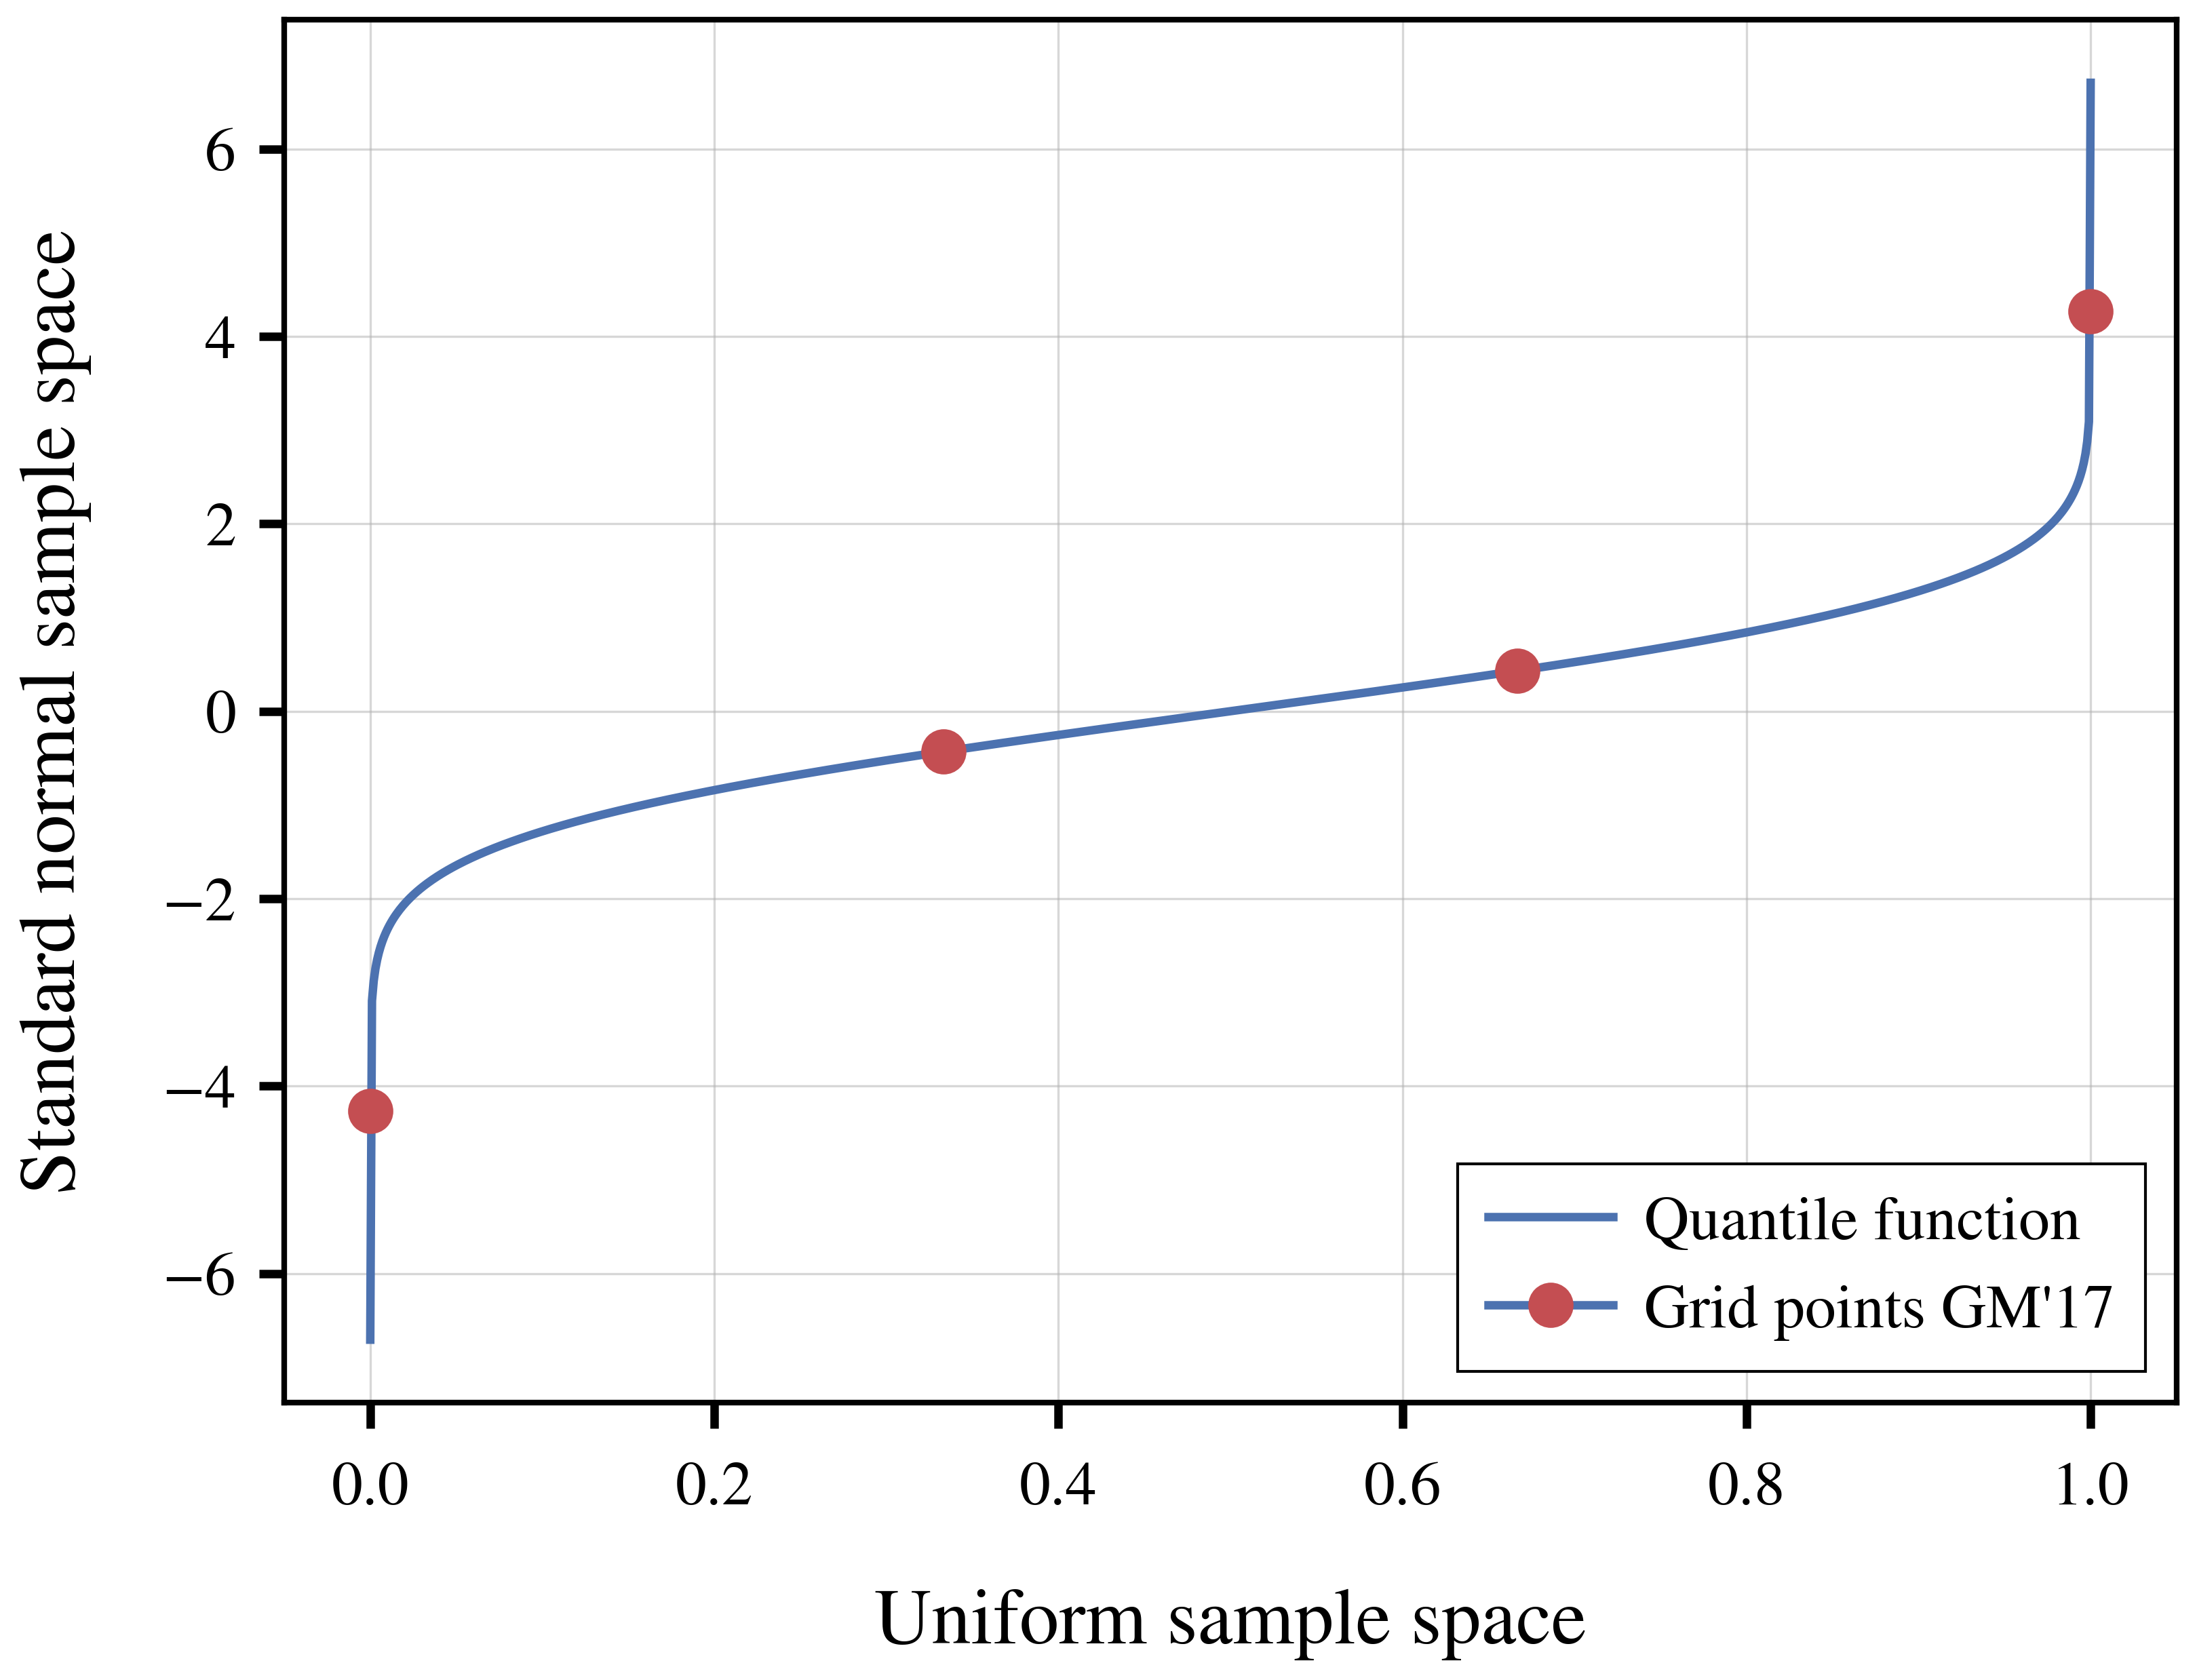
\includegraphics[scale=0.40]{../../../scrypy/figures/quantile_fct}
	\label{fig:rad}
\end{figure}



\newpage
\begin{figure}[H]
	\caption{Sigma-normalized mean absolute Elementary Effects for trajectory design}
	\centering
	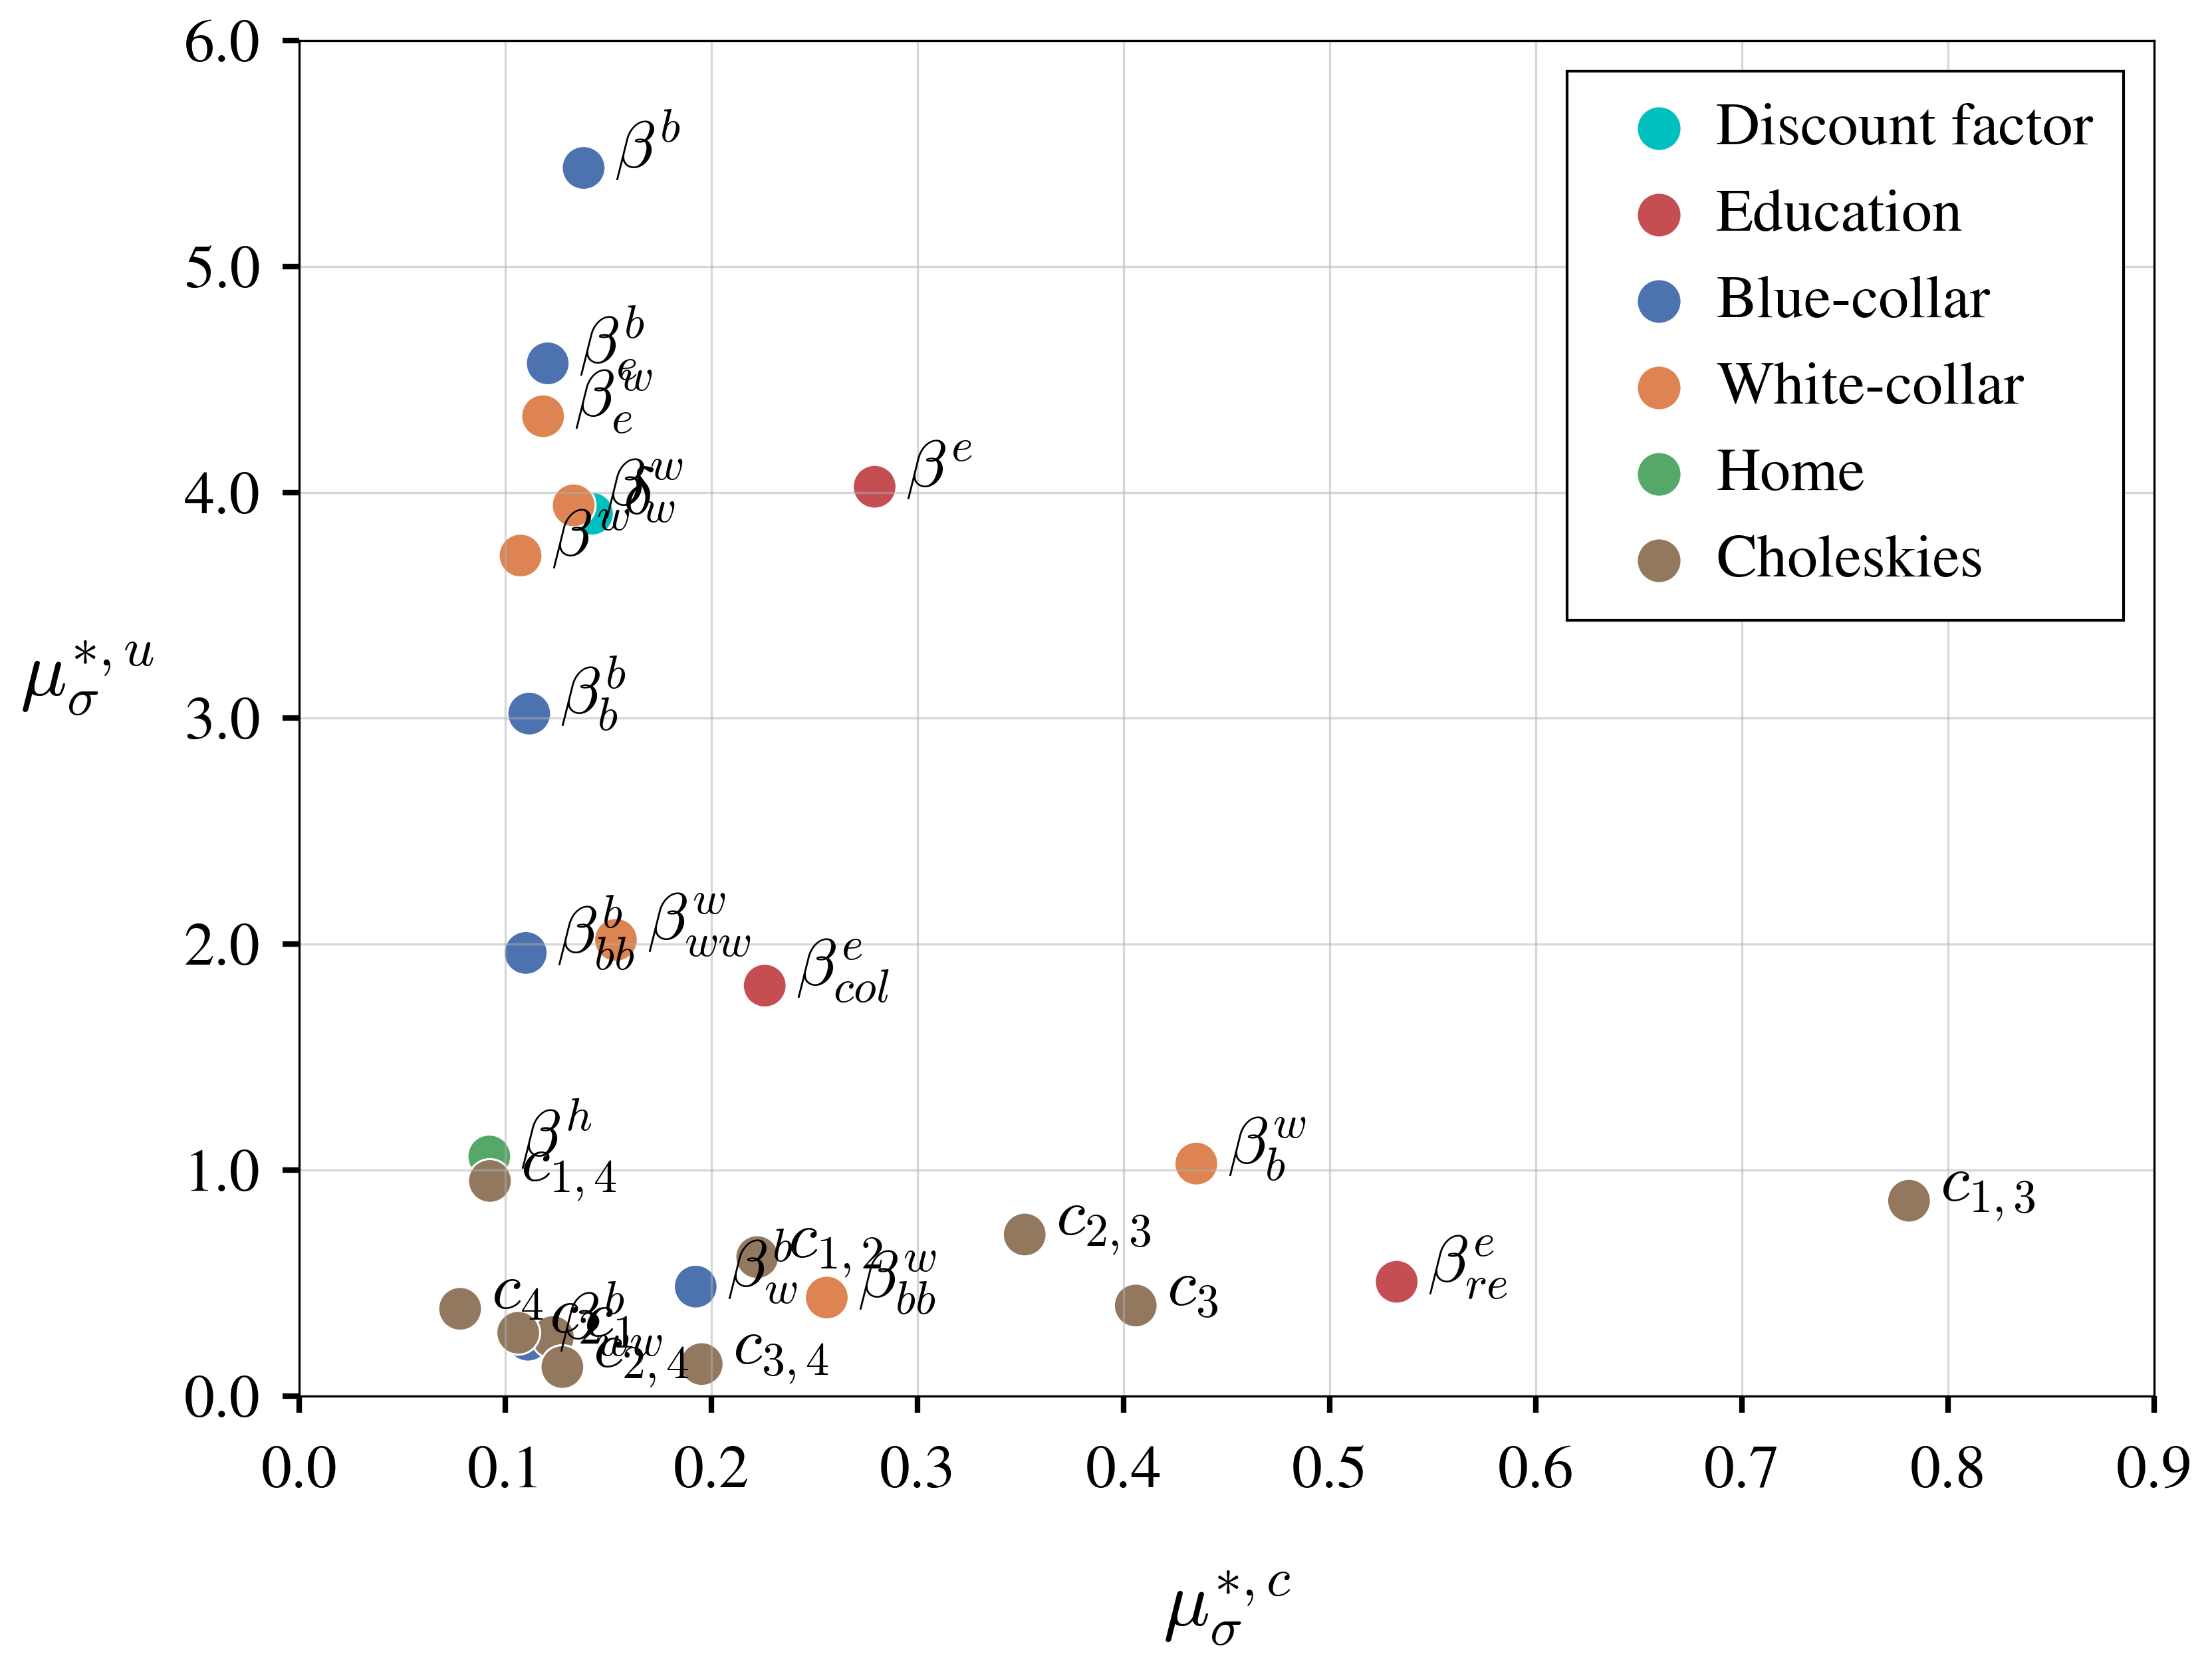
\includegraphics[scale=0.52]{../../../scrypy/figures/scatter_traj}
	\label{fig:traj}
\end{figure}

\begin{figure}[H]
	\caption{Sigma-normalized mean absolute Elementary Effects for radial design}
	\centering
	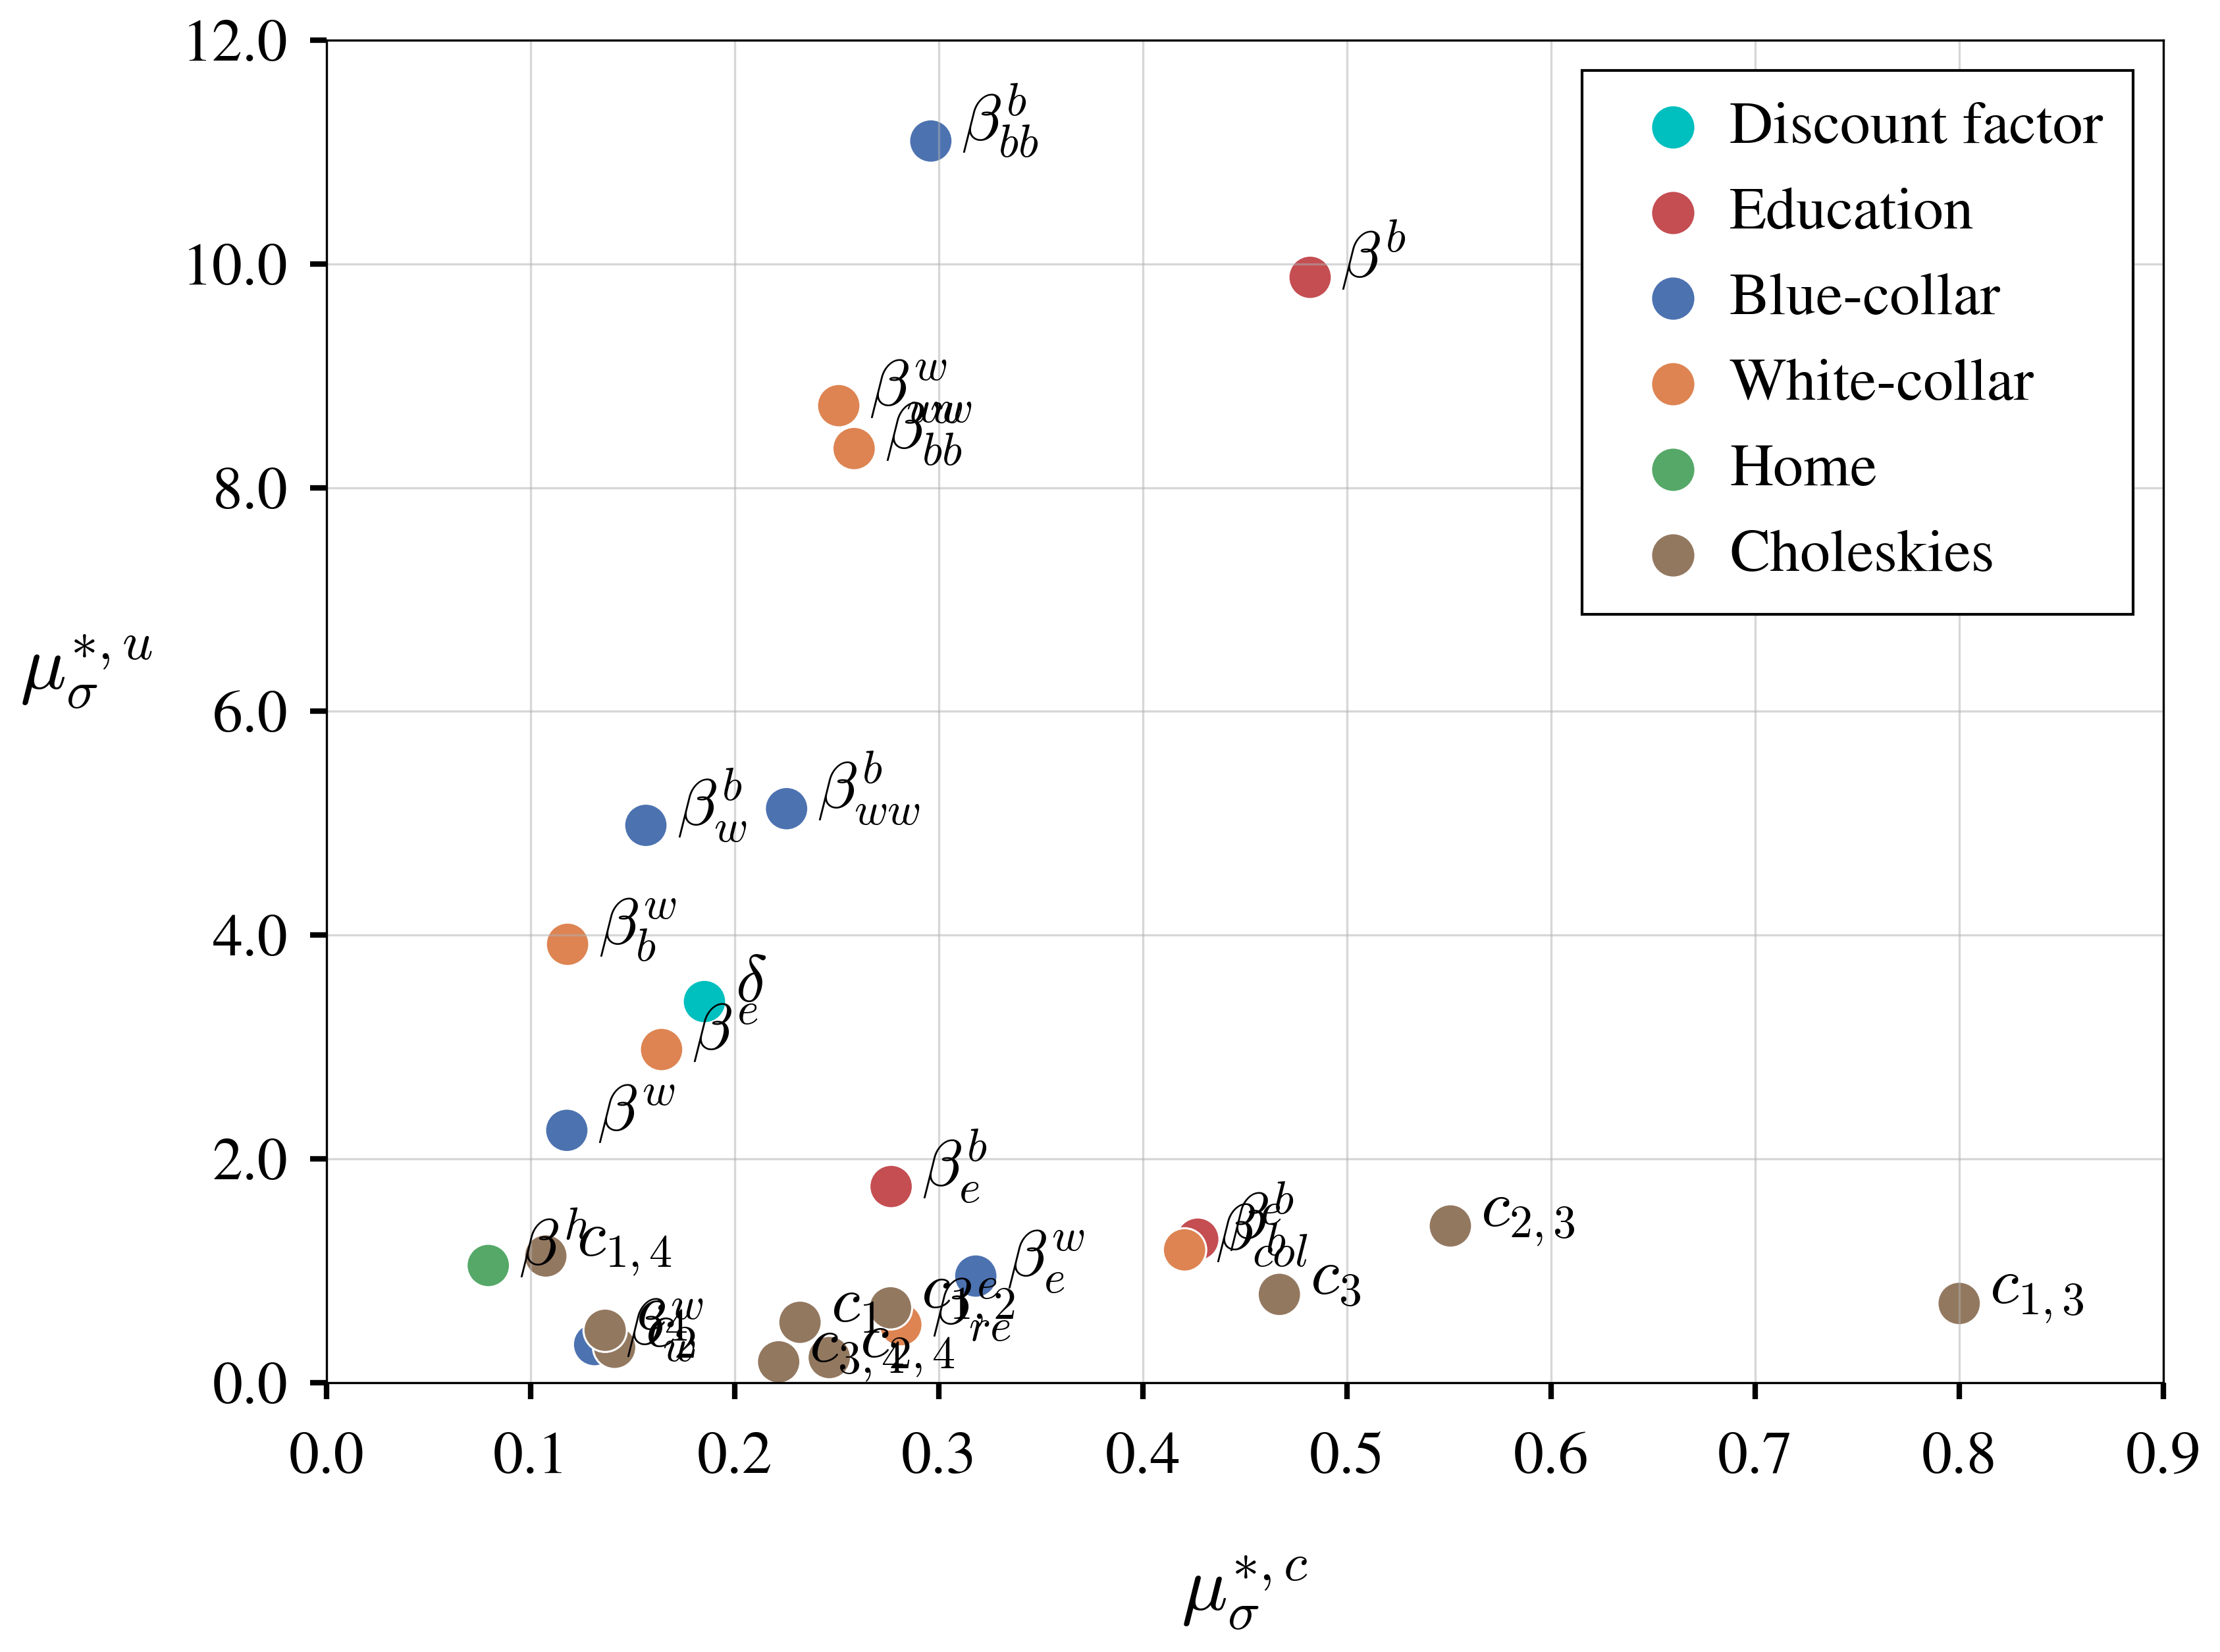
\includegraphics[scale=0.52]{../../../scrypy/figures/scatter_rad}
	\label{fig:rad}
\end{figure}



\newpage
\bibliography{../../bibliography/literature}

\end{document}